% !TeX root=main.tex
% دستور زیر باید در اولین فصل شما باشد. آن را حذف نکنید!

\chapter{مروری بر ادبیات}
\thispagestyle{empty}

در فصل پیش، به معرفی فضای یادگیری در جریان‌های داده‌ای پرداختیم  و ویژگی‌های این الگوریتم‌ها و محیط اجرای آن‌ها  را بررسی کردیم. همچنین مقایسه‌ای از محدودیت‌های این الگوریتم‌ها با الگوریتم‌های سنتی ارایه دادیم. در این فصل به مقدمات اصلی کار می‌پردازیم و تعاریفی نظیر مفهوم، منبع داده، رانش مفهوم و پنجره‌ی زمانی را مطرح می‌کنیم. به علاوه رویکردهای کلی به الگوریتم‌های یادگیری محیط داده‌های جریانی را نیز بررسی خواهیم کرد و در نهایت نرم‌افزارها و داده‌های مورد استفاده در فضای تحقیقاتی را معرفی خواهیم کرد.  

\section{تعاریف اولیه}\label{sec2}
در این بخش به معرفی چند تعریف اولیه نظیر منبع داده، مفهوم، رانش مفهوم می‌پردازیم.
\subsection{جریان داده}
یک جریان داده \LTRfootnote{Data Stream} به شکل یک دنباله از نمونه‌های داده تعریف می‌شود\cite{kelly1999impact} و آن را با نماد $DS$ نشان می‌دهیم:
$DS = \left\{ x_1, x_2, ..., x_t, ...\right\}$
که در این رابطه $x_i$ برابر i امین داده‌ی مشاهده شده است. هر نمونه داده‌ی $x_i$ یک برچسب دارد و با  $ y_i \in Y = \left\{y_1, y_2, ..., y_c\right\} $ نشان داده می‌شود.


\subsection{مفهوم}
یک مفهوم\LTRfootnote{Concept} یا یک منبع داده، توسط احتمال پیشین برای رده‌ها و تابع توزیع احتمال رده‌‌ی آن ها تعریف می‌شود\cite{kelly1999impact}:

$$
S = \left\{(P(y_1), P(X|y_1));...;(P(y_c), P(X|y_c))\right\} 
$$
که در این رابطه y بیانگر رده‌ها است. روش‌های سنتی یادگیری ماشین و داده‌کاوی با یک مفهوم کار می‌کند، و این بدان معنی است که تابع توزیع احتمال مجموعه آموزش و مجموعه آزمون یکسان است. این در حالی است که داده‌های جریانی پویا هستند و تعداد زیادی مفهوم دارند. یک مثال از این تغییر مفهوم را می‌توانید حمله‌ی هکری در یک شبکه‌ی کامپیوتری را در نظر بگیرید\cite{Nguyen2015}
. توضیح مفهوم داده‌ی «معمولی» با داده‌ی «حمله» در طی زمان تغییر می‌کند. همیشه حمله‌ها در حال انجام هستند ولی انواع و روش‌های آن تغییر می‌کند.
\\
یک جریان داده‌ای مانند DS شامل یک مجموعه k عضوی از منبع داده را در نظر بگیرید که در آن منابع داده با $S_i$ نشان‌ داده می‌شود و توزیع این منابع شناخته شده است( $ i = 1, ..., k $ ). در زمان t یک یا چند منبع داده فعال وجود دارد. فرض کنید $w_i(t) \in [0, 1]$ برابر با تاثیر منبع داده  $S_i$ در زمان t باشد. توزیع داده‌ی جریان داده‌ی DS در زمان t توسط رابطه زیر مشخص می‌شود\cite{kelly1999impact}:
$$
\sum^{DS}(t) = \left\{ w(1)S_1, ..., w(k)S_k \right\}
$$

\begin{figure}%[ht]
\centerline{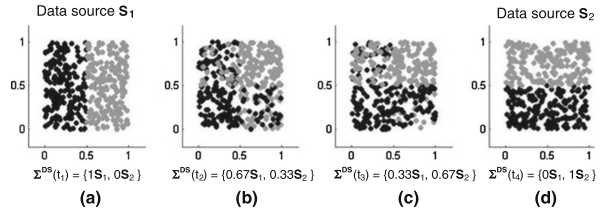
\includegraphics[width=15cm]{drift}}
\caption{مثالی از تغییر تدریجی منبع $S_1$ به منبع $S_2$. در این شکل کلاس $ y_1 $ با رنگ خاکستری و کلاس $ y_2 $ با رنگ مشکی مشخص شده است\cite{narasimhamurthy2007framework}.}
\label{fig:drift}
\end{figure}




\subsection{رانش مفهوم}

 اگر فرض کنیم که یک منبع داده DS شامل k منبع جریانی مستقل S با وزن اثر w باشد، اگر در دو زمان $t_1$ و $t_2$ رابطه زیر برقرار باشد می گوییم رانش مفهوم \LTRfootnote{Concept Drift} رخ داده است.
\begin{equation}
\sum^{DS}(t_1) \neq \sum^{DS}(t_2)
\label{eq:drift}
\end{equation}

در تصویر
\ref{fig:drift}
می‌توانید یک نمونه از رانش مفهوم که بصری‌سازی شده است را طی زمان‌های مختلف مشاهده کنید.

بر اساس رابطه
\ref{eq:drift}
هر نوع تغییری(حتی کوچک‌ترین تغییرات) در منبع جریان، یک رانش مفهوم حساب می‌شود. بنابراین رانش‌های مفهوم را به دو دسته اساسی تقسیم می‌کنیم
\cite{bouguelia2016adaptive}:


\subsubsection{رانش مفهوم مجازی}
اگر رانش مفهوم تأثیر مستقیمی بر حدود تصمیم‌گیری نداشته باشد(احتمال پیشین داده‌ها تغییر نکند) اما رانش بر روی تابعِ چگالی احتمال اثر بگذارد، گوییم که رانش مفهوم مجازی \LTRfootnote{Virtual Concept Drift} رخ داده است.

\subsubsection{رانش مفهوم حقیقی}
اگر رانش مفهوم علاوه بر تغییر تابع چگالی احتمال، تأثیر مستقیم بر حدود تصمیم‌گیری بگذارد و احتمال‌های پیشین را تغییر دهد، گوییم رانش مفهوم حقیقی \LTRfootnote{Real Concept Drift} رخ داده است. روش‌های یادگیری در محیط‌های جریان‌های داده‌ای باید به گونه‌ای باشند که با رانش مفهوم حقیقی سریعا سازگار شوند.


\section{پنجره‌های زمانی}
از آن‌جایی که داده‌های جریانی امکان دارد بینهایت باشند، تنها مقدور است که بخشی از تمام داده‌ی جریانی را پردازش کنیم. این بخش مورد توجه از داده توسط یک پنجره زمانی از نمونه‌های داده تعریف می‌شود.
\begin{equation}
W[i, j] = (x_i, x_{i+1}, ..., x_j)
\end{equation}
بر اساس این تعریف، انواع مختلفی از پنجره زمانی بیان‌ می‌شود: پنجره نقطه عطفی
\LTRfootnote{Landmark Window}
،پنجره کشویی
\LTRfootnote{Sliding Window}
،پنجره محو شونده
\LTRfootnote{Fading Window}
و پنجره یک‌بر
\LTRfootnote{Tilted Window}.

\subsection{پنجره نقطه عطفی}
در پنجره نقطه عطقی، ما به تمام داده جریانی از زمان شروع نمونه اول تا زمان فعلی نمونه $ t_c $ توجه می‌کنیم: پنجره به شکل $ W[1, c] $ تعریف می‌شود\cite{domingos2000mining}. استفاده از پنجره نقطه عطفی بدین معناست که تمامی تراکنش‌ها در پنجره به شکل یکسانی برای ما اهمیت دارند؛ هیچ تفاوتی داده‌های گذشته و حال وجود ندارد. به طور مداوم که داده‌های جریانی تغییر می‌کنند، مدل با استفاده از داده قدیمی نمونه‌ها ساخته می‌شود که حتی ممکن است که با داده‌های جدید ناسازگار باشند. برای تاکید بیشتر روی داده‌های جدیدتر می‌توان از پنجره‌های کشویی، محوشونده و یک بر استفاده کرد.

\subsection{پنجره کشویی}
   در پنجره کشویی که با
$W[t_c - w + 1, t_c]$
 نشان داده می‌شود ما تنها به w تراکنش اخیر توجه می‌کنیم و بقیه داده‌های جریانی نادیده گرفته‌ می‌شوند\cite{nguyen2012heterogeneous}. نتیجه کاوش وابسته به اندازه پنجره است که w بیانگر آن است. اگر w خیلی بزرگ باشد و رانش مفهوم رخ دهد، پنحره ممکن است شامل داده‌‌ها و اطلاعات منقضی شده باشد و دقت مدل کاهش پیدا می‌کند. اگر w کوچک باشد، پنجره ممکن است شامل داده‌های ناکارامد باشد و مدل دچار بیش‌برازش گردد.
کارهای قبلی یک مقدار ثابت را برای اندازه پنجره کشویی در نظر‌ می‌گرفتند که توسط کاربران و با آزمایش تعیین می‌شد. اخیرا چند کار \cite{bifet2010adaptive} برای ارایه پنجره کشویی انعطاف پذیر ارایه شده است که در آن اندازه پنجره بر اساس دقت مدل تغییر می‌کند؛ زمانی که دقت زیاد باشد اندازه پنجره بزرگ می‌شود و زمانی هم که دقت کم شود، پنجره کوچک می‌شود.


\subsection{پنجره محوشونده}
در پنجره‌های محو شونده، هر نمونه از داده‌های جریانی با یک وزن که با زمان رسیدن آن نمونه در ارتباط است شناسایی می‌شود؛ بنابراین داده‌هایی که جدیدتر می‌رسند، وزن بیشتری از داده‌های قدیمی‌تر دارند\cite{leite2009evolving}. با استفاده از پنجره محو شونده، می‌توان تاثیر(اهمیت) داده‌های قدیمی منقرض شده را کاهش داد تا در نتیجه کاوش تاثیری نداشته باشند. معمولا از یک تابع نمایی نزولی مانند تابع زیر برای پنجره زمانی استفاده می‌شود:
$$
f(\triangle t) = \lambda^{\triangle t}(0 < \lambda < 1)
$$
که در این تابع $\triangle t$ قدمت(سن) نمونه داده‌ی جریانی و برابر با تفاوت زمانی فعلی و زمان مشاهده داده است. پنجره محو شونده نیاز به انتخاب یک پارامتر محوشوندگی مانند $ \lambda $ دارد که معمولا یک عدد در بازه $ [0.99, 1] $ برای کاربردهای واقعی انتخاب می‌شود\cite{Nguyen2015}.


\subsection{پنجره یک‌بر}
پنجره یک‌بر یک نوع پنجره زمانی شبیه پنجره محو شونده و کشویی است\cite{aggarwal2006framework}. این پنجره در سطوح مختلف ریزدانگی که با توجه به تاخر داده شکل گرفته‌اند اعمال می‌شود. پنجره زمانی‌ یک‌بر تقریبا تمام مجموعه داده را ذخیره کرده و یک تعادل بین فضای مورد نیاز برای ذخیره‌سازی و دقت برقرار می‌کند. البته این‌ مدل می‌تواند پس از اجرای طولانی غیر پایدار باشد.



\begin{figure}%[ht]
\centerline{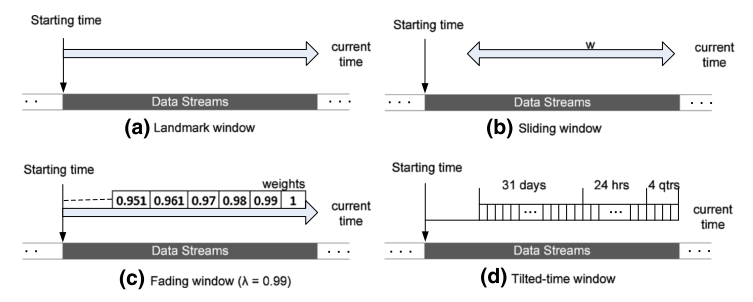
\includegraphics[width=15cm]{time-windows}}
\caption{پنجره‌های مختلف زمانی}
\label{fig:time-windows}
\end{figure}
تصویر
\ref{fig:time-windows}\cite{Nguyen2015}
چهار نوع مختلف پنجره زمانی را نشان می‌دهد. برای پنجره محو شونده $\lambda$ برابر با $0.99$ تنظیم شده است و وزن نمونه‌ها کاهش می‌یابد. برای پنجره یک‌بر، ما جهار ربع اخیر یک ساعت را ذخیره کرده‌ایم، سپس ۲۴ ساعت گذشته و ۳۱ روز اخیر نمایش داده شده‌اند.



\begin{figure}%[ht]
\centerline{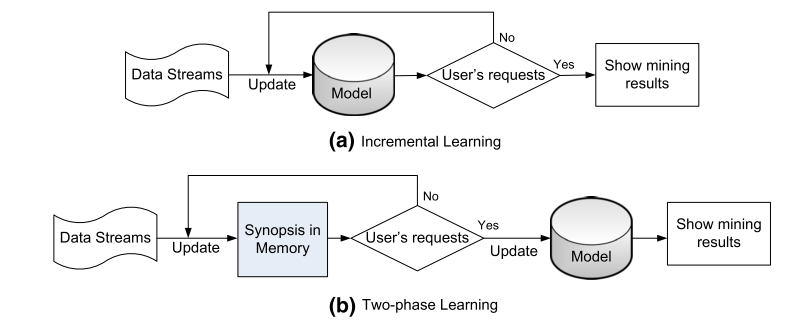
\includegraphics[width=15cm]{approach}}
\caption{الف- رویکرد افزایشی به یادگیری. ب- رویکرد دو گامی}
\label{fig:approach}
\end{figure}


\section{رویکردهای محاسباتی}

براساس انواع مختلف پنجره زمانی، دو رویکرد محاسبانی مختلف برای پردازش داده‌های جریانی وجود دارد.

\subsection{یادگیری افزایشی}
یادگیری افزایشی\LTRfootnote{Incremental Learning} یک رویکرد محاسباتی برای داده‌های جریانی است\cite{seidl2009indexing}. در این رویکرد، مدل به صورت افزایشی تغییری می‌کند تا با تغییرات در داده‌هایی که در حال آمدن هستند، سازگار شوند. دو طرح کلی برای بروزرسانی مدل وجود دارد: بروزرسانی با هر نمونه داده و بروزرسانی با پنجره. به عنوان نمونه ستریت
\LTRfootnote{Street}
و همکارانش \cite{street2001streaming}یک مجمع از رده‌بندها برای داده‌های جریانی توسعه‌ دادند که یک پنجره از داده‌های ورودی را می‌گیرد و مدل را با تنظیم وزن‌های هر رده‌بند یا جایگزین کردن رده‌بند‌های قدیمی با نمونه‌های جدیدشان سازگار می‌کند. شکل
\ref{fig:approach}
- الف رویکرد یادگیری افزایشی را نمایش می‌دهد. مزیت این رویکرد این است که نتیجه برای هر نمونه(یا پنجره‌ای از نمونه‌ها) در دسترس است ولی به منبع محاسباتی بیشتری نیاز است.
\subsection{یادگیری دوگامی}
یادگیری دوگامی\LTRfootnote{Two-Phase Learning}، که با نام یادگیری آنلاین-آفلاین نیز شناخته می‌شود یک رویکرد محاسباتی برای داده‌های جریانی است\cite{aggarwal2006framework}. ایده‌ بنیادی این است که کاوش بر داده‌ها را به دو بخش تقسیم کنیم. در گام اول(گام آنلاین)، چکیده‌ای از داده در لحظه ایجاد می‌شود. در گام دوم(گام آفلاین)، بر مبنای درخواست کاربر، پردازش روی چکیده‌هایی که در گام قبل ایجاد شده بود انجام می‌شود.
به عنوان مثال، آگراول
\LTRfootnote{Aggarwal}
 و همکارانش\cite{aggarwal2003framework}، یک روش آنلاین-آفلاین برای خوشه‌بندی داده‌های جریانی ارایه کرده‌اند که در بخش آنلاین، خلاصه‌ای از اطلاعات آماری داده جریانی به صورت برخط گردآوری می‌شود. در طول بخش آفلاین، از این داده‌ها برای خوشه بندی سطح بالا استفاده می‌شود. رویکرد یادگیری دوگامی در شکل نشان داده شده است. این روش قابلیت پردازش داده های جریانی را با سرعت بیشتری داد منتها محدودیت آن این است که کاربر باید تا فراهم شدن نتیجه، منتظر بماند.
شکل
\ref{fig:approach}
- ب رویکرد یادگیری آنلاین-آفلاین را نمایش می‌دهد.




\section{اعتبار سنجی}
در روش‌های سنتی یادگیری ماشین با مقدار داده‌ی محدود، فرآیند اعتبارسنجی بر استفاده‌ی بیشینه از داده تمرکز داشت. جداسازی
\LTRfootnote{Hold-out}،
اعتبار سنجی متقابل
\LTRfootnote{Cross-Validation}
و تک‌گذاری
\LTRfootnote{Leave-One-Out}
روش‌های استاندارد اعتبار سنجی هستند. در روش جداسازی به شکل تصادفی مجموعه‌ی داده به دو زیر مجموعه، یکی برای آموزش و دیگری برای آزمایش تقسیم می‌شود؛ نسبت‌های رایج برای تقسیم داده به مجموعه آموزش و آزمایش نصف و یک‌سوم است. در روش اعتبار سنجی متقابل با k دسته، داده به k مجموعه‌ی مساوی و مستقل از نمونه‌ها تقسیم می‌شد و یکی از این زیر مجوعه‌ها برای آزمایش و باقی آن‌ها( $k-1$ )برای آموزش ادغام می‌شد؛ در این روش فرآیند اعتبارسنجی k بار و هر بار با یک زیر مجموعه برای آزمایش انجام می‌شود. روش تک‌گذاری نیز یک نوع اعتبار سنجی متقابل است که در آن k با تعداد کل داده‌ها برابر است.
\\
در محیط جریان‌های داده‌ای، از آن‌جایی که داده می‌تواند نامحدود باشد، اعتبار سنجی بر ارزیابی مدل در صحنه‌های مختلف متمرکز است\cite{Nguyen2015}. یک روش شناخته‌شده رسم منحنی یادگیری با ذخیره‌سازی کارایی مدل در طول زمان است؛ این منحنی نشان‌ خواهد داد که چقدر مدل پس از مشاهده‌ی داده‌های بیشتر، بهتر شده است و مدل چگونه با رانش‌ مفهوم سازگار می‌شود. یک الگوریتم برتری خود را به سایر روش‌ها زمانی نشان می‌‌دهد که منحنی یادگیریش بیشتر مواقع از سایر الگوریتم‌ها بالا‌تر باشد.
\\
روش جداسازی و روش پی‌درپی
\LTRfootnote{Prequential}
دو روش پر کاربرد برای اعتبارسنجی جریان‌های داده‌ای هستند\cite{Nguyen2015}. در روش جداسازی، نمونه‌های داده به چانک‌های مختلفی تقسیم می‌شوند؛ از هر چانک داده ابتدا برای آزمایش و سپس برای بروزرسانی مدل استفاده می شود. روش جداسازی زمانی که رانش‌ مفهوم رخ داده، ترجیح داده می‌شود چون این روش اجازه می‌دهد که مدل با آخرین تغییرات داده سازگار شود. روش پی‌در‌پی(یا آزمایش-سپس-آموزش
\LTRfootnote{Test-Then-Train}
به شکل لایه‌ لایه) یک روش دیگر برای ارزیابی جریان‌های داده‌ای است\cite{bifet2010moa}. هر نمونه داده ابتدا و پیش از این‌که برای آموزش به صورت افزایشی استفاده شود، برای آزمایش استفاده می‌شود. این روش می‌تواند یک حالت خاص برای روش جداسازی در نظر گرفته شود اگر اندازه چانک برابر با یک باشد. مزیت این روش این است که نیازی به تعریف از پیش اندازه چانک نیست ولی متاسفانه کارایی این الگوریتم در زمان محدود  مبهم است چراکه اشتباهات اولیه مدل به سرعت در طول زمان کاهش می‌یابد.


\subsubsection{معیارهای ارزیابی}


به طور عمومی معیارهای ارزیابی روش‌های سنتی یادگیری ماشین، می‌تواند برای ارزیابی یادگیرنده‌ها در جریان‌های داده نیز استفاده شود. برای رده‌بندی داده‌ها، صحت
\LTRfootnote{Accuracy}
و تابع ضرر $0-1$ دو معیار رایج هستند. برای ارزیابی مداوم کارایی رده‌بندی در داده‌های جریانی، گیم
\LTRfootnote{Gama}
و همکارانش \cite{gama2007learning} یک روش ضرر پی‌در‌پی که با انواع مختلف پنجره کار می‌کند را ارایه کرده‌اند. برای از یاد‌بردن پی‌در‌پی خطا اثبات شده است که همگرایی خطای بیز در داده‌های ایستا، روش را برای تشخیص رانش کارا می‌سازد. این روش می‌تواند به سادگی روی سایر معیار‌های کارایی نیز اعمال شود.

\section{نرم‌افزارهای کاربردی}
نرم‌افزارهای مختلف کاربری و متن‌باز برای تحقیقات دانشگاهی در حوزه‌ی یادگیری و داده‌کاوی در محیط‌های پویای جریان‌های داده‌ای وجود دارد.

\subsubsection{WEKA}
شناخته‌شده‌ترین ابزار داده‌کاوری در محیط دانشگاهی است. این ابزار شامل یک مجوعه از الگوریتم‌های پردازی داده، رده‌بندی، رگرسیون، خوشه‌بندی، قواعد باهم‌آیی و بصری سازی داده است\cite{hall2009weka}.

\subsubsection{MOA}
نرم افزار MOA \cite{bifet2010moa}
یک فریمورک متن‌باز محبوب برای داده کاوی در داده های جریانی است که توسط دانشگاه وایکیتو نیوزلند
\LTRfootnote{University of Waikato, New Zealand}
 و بر مبنای چهارچوب  WEKA توسعه داده شده است. در این نرم افزار که توسط زبان جاوا پیاده سازی شده، تعداد زیادی ابزار مناسب جهت پیاده سازی و تست الگوریتم های یادگیری و خوشه بندی و تشخیص رانش مفهوم وجود دارد. برای نمونه الگوریتم‌های درخت‌ تصمیم خیلی سریع و مجمع رده‌بند ها که در ادامه توضیح داده‌ می‌شوند در این چهارچوب موجود است.
این ابزار تعدادی تولید‌‌کننده
\LTRfootnote{Generator}
 داده جریانی مانند مفهوم‌های SEA  ،ابرصفحه‌ی دوران کننده
\LTRfootnote{Rotating Hyperplane}
 و STAGGER را فراهم کرده است.
\subsubsection{Rapid-Miner}
یکی دیگر از ابزارهای متن‌باز برای داده‌کاوی است\cite{hofmann2013rapidminer}. RapidMiner بسیار قدرتمندتر از WEKA است و تمام الگوریتم‌های WEKA و سایر الگوریتم‌های پیشرفته را دارد. این ابزار خلاقانه‌تر است و این قابلیت را داد که پروسه داده‌کاوی را به شکل یک دنباله از عملگرها تعریف کرد. همچنین RapidMiner ابزارهای بیشتری را بصری‌سازی فراهم کرده است.
\section{مخزن‌های داده}
داده‌های واقعی بسیار کمی برای ارزیابی روش‌های یادگیری در داده‌های جریانی وجود دارد\cite{Nguyen2015}. یک دلیل این ‌موضوع می‌تواند این باشد که محققان روش‌های سنتی داده‌کاوی و یادگیری ماشین معمولا داده‌های خود را به قدری کوچک نگه‌می‌داشتند تا با روش‌های یادگیری دسته‌ای
\LTRfootnote{Batch Learning}
سازگار باشد.
\\

 یک دلیل دیگر می‌تواند مساله حریم شخصی در انتشار داده‌های که خیلی بزرگ هستند باشد. محققان معمولا از داده‌های خصوصی برای اثبات سیستم‌هایشان استفاده می‌کنند که نمی‌توانند آن‌ها را منتشر کنند. برای غلبه بر این کمبود، بعضی از مجموعه داده‌های ترکیب شده با تعداد نامحدود داده ساخته شده‌اند. برای مثال تولید کننده ‌درخت تصادفی، تولید‌ کننده مفهوم SEA و ابرصفحه‌های چرخنده تولید شده‌اند. این تولیدکننده‌های داده در چهارچوب MOA پیاده‌سازی شده‌اند\cite{bifet2010moa}.
 
 
برای جریان‌های متنی تقریبا می‌توان گفت که داده‌ای که تمام ویژگی‌های داده‌های جریانی و داده‌های متنی را داشته باشد در دسترس نیست. به علاوه از تولید‌کننده‌ها نمی‌توان برای تولید داده‌های متنی استفاده کرد. تولید داده‌های متنی مناسب، که حجم زیادی داشته‌ باشد و در آن رانش مفهوم مکررا اتفاق افتاده باشد یک چالش اساسی برای ادامه تحقیقات در این حوزه است ولی برای کاربرهای دیگر بعضی از مخزن‌های داده با مجموعه‌های داده‌ی بزرگ نیز برای ارزیابی روش‌های یادگیری در داده‌های جریانی استفاده می شود:
\subsubsection{\lr{UCI Machine Learning Repository}}
یک مخزن آنلاین معتبر\LTRfootnote{http://www.ics.uci.edu/~mlearn/mlrepository.html}  و شناخته شده برای آزمایش و آنالیز الگوریتم‌های یادگیری ماشین است. سه مجموعه داده پر استفاده در چندین مقاله برای ارزیابی جریان‌ها Forest Covertype و Poker-Hand و Electricity هستند\cite{Nguyen2015}.
\subsubsection{\lr{KDD Cup Center}}
رقابت‌های سالانه‌ی داده‌کاوی و کاوش دانش توسط
\lr{ACM Special Interest Group\LTRfootnote{http://www.kdd.org/}}
سازمان‌دهی می‌شود. معمولا داده‌هایی که برای این رقابت تولید می‌شود می‌تواند منبع خوبی برای ارزیابی الگوریتم‌های یادگیری ماشین در داده‌های جریانی باشد.
